%%%%%%%%%%%%%%%%%%%%%%%%%%%%%%%%%%%%%%%%%%%%%%%%%%%%%%%%%%%%%%%%%%%%%%%%%%%%%%%
%  Summary slides -- what I work on, and a rapid overview of Lean
%  Joseph Tooby-Smith -- University of Bath
%
%  Compile with: pdflatex SummarySlide.tex
%%%%%%%%%%%%%%%%%%%%%%%%%%%%%%%%%%%%%%%%%%%%%%%%%%%%%%%%%%%%%%%%%%%%%%%%%%%%%%%
\documentclass[aspectratio=169,10pt]{beamer}

\usepackage[T1]{fontenc}
\usepackage[utf8]{inputenc}
\usepackage[sfdefault]{FiraSans}
\usefonttheme[onlymath]{serif}
\usepackage{amsmath,amssymb}
\usepackage{tikz}
\usepackage{listings}
\usepackage{fontawesome5}
\usepackage[most]{tcolorbox}
\usetikzlibrary{arrows.meta}

\hypersetup{colorlinks=false, pdfborder={0 0 0}}

%%%%%%%%%%%%%%%%%%%%%%%%%%%%%%%%%%%%%%%%%%%%%%%%%%%%%%%%%%%%%%%%%%%%%%%%%%%%%%%
%  PALETTE  (PhysLib house style)
%%%%%%%%%%%%%%%%%%%%%%%%%%%%%%%%%%%%%%%%%%%%%%%%%%%%%%%%%%%%%%%%%%%%%%%%%%%%%%%
\definecolor{plnavy}  {HTML}{24476B}
\definecolor{plblue}  {HTML}{3D6B99}
\definecolor{plsky}   {HTML}{6FA3CE}
\definecolor{plorange}{HTML}{EF6B3B}
\definecolor{plgreen} {HTML}{3FA56A}
\definecolor{plink}   {HTML}{243447}
\definecolor{plmuted} {HTML}{5C7187}
\definecolor{plrule}  {HTML}{C7DCED}
% plorange is a fill/icon colour: too light to set small text on white.
% plember is its text-weight sibling, used wherever orange has to be read.
\definecolor{plember} {HTML}{B0421B}

%%%%%%%%%%%%%%%%%%%%%%%%%%%%%%%%%%%%%%%%%%%%%%%%%%%%%%%%%%%%%%%%%%%%%%%%%%%%%%%
%  BEAMER FURNITURE  (plain white slide)
%%%%%%%%%%%%%%%%%%%%%%%%%%%%%%%%%%%%%%%%%%%%%%%%%%%%%%%%%%%%%%%%%%%%%%%%%%%%%%%
\setbeamertemplate{navigation symbols}{}
\setbeamercolor{background canvas}{bg=white}
\setbeamersize{text margin left=0.62cm,text margin right=0.62cm}
\setbeamercolor{normal text}{fg=plink}
\setbeamercolor{frametitle}{fg=plnavy}
\setbeamercolor{itemize item}{fg=plblue}
\setbeamerfont{frametitle}{size=\LARGE,series=\bfseries}
\setbeamertemplate{itemize item}{\raisebox{0.15ex}{\tiny$\blacksquare$}}
\setlength{\leftmargini}{1.2em}

\setbeamertemplate{frametitle}{%
  \vspace*{0.34cm}%
  \begin{minipage}{\dimexpr\paperwidth-1.4cm\relax}
    \raggedright
    {\usebeamerfont{frametitle}\usebeamercolor[fg]{frametitle}\insertframetitle\par}
    \vspace{4pt}
    {\color{plorange}\rule{1.4cm}{2.4pt}}{\color{plrule}\rule{\dimexpr\linewidth-1.4cm\relax}{2.4pt}}
  \end{minipage}\par\vspace{0.16cm}%
}

\newcommand{\plbody}{\small}
\newcommand{\plmeta}{\footnotesize}
\newcommand{\pllabel}{\footnotesize\bfseries}

%%%%%%%%%%%%%%%%%%%%%%%%%%%%%%%%%%%%%%%%%%%%%%%%%%%%%%%%%%%%%%%%%%%%%%%%%%%%%%%
%  CARDS
%%%%%%%%%%%%%%%%%%%%%%%%%%%%%%%%%%%%%%%%%%%%%%%%%%%%%%%%%%%%%%%%%%%%%%%%%%%%%%%
\tcbset{
  plbase/.style={
    enhanced, arc=6pt, outer arc=6pt, boxrule=0pt, leftrule=4pt,
    colback=white, left=10pt, right=10pt, top=8pt, bottom=8pt,
    halign=flush left,
    drop fuzzy shadow={black!25}, before skip=4pt, after skip=4pt,
  }
}
% Each argument: [extra tcolorbox options] {accent colour} {heading}
\newtcolorbox{plcard}[3][]{plbase, colframe=#2, #1,
  before upper={{\bfseries\color{#2}#3}\par\vspace{5pt}}}
\newtcolorbox{plplain}[2][]{plbase, colframe=#2, #1}

%%%%%%%%%%%%%%%%%%%%%%%%%%%%%%%%%%%%%%%%%%%%%%%%%%%%%%%%%%%%%%%%%%%%%%%%%%%%%%%
%  LEAN LISTINGS  (ASCII-only source, so pdflatex stays happy)
%%%%%%%%%%%%%%%%%%%%%%%%%%%%%%%%%%%%%%%%%%%%%%%%%%%%%%%%%%%%%%%%%%%%%%%%%%%%%%%
\lstdefinelanguage{lean}{
  morekeywords={theorem,lemma,def,abbrev,example,structure,instance,class,where,
    by,fun,have,show,from,let,match,with,namespace,end,open,variable,
    intro,exact,apply,simp,rfl,ring,unfold,positivity,sorry,Type,Prop,Sort,
    induction,rw,at,
    inductive,cases,Empty,Ne,Nat},
  sensitive=true,
  morecomment=[l]{--},
  morecomment=[s]{/-}{-/},
  morestring=[b]",
}
\lstset{
  language=lean,
  basicstyle=\ttfamily\small\color{plink},
  keywordstyle=\bfseries\color{plnavy},
  commentstyle=\itshape\color{plgreen!80!black},
  showstringspaces=false,
  columns=fullflexible,
  breaklines=false,
  aboveskip=1pt, belowskip=1pt,
}

\newcommand{\plchip}[2]{%
  \tikz[baseline=(t.base)]{\node[fill=#1!85!black,text=white,rounded corners=5pt,
    inner xsep=5pt,inner ysep=1.8pt,font=\bfseries\scriptsize] (t) {#2};}}

% A square GitHub repository card.
\newtcolorbox{plsquare}{enhanced, nobeforeafter, box align=center,
  width=3.8cm, height=3.8cm, valign=center, halign=flush left,
  arc=10pt, outer arc=10pt, colback=white, colframe=plrule, boxrule=1.2pt,
  left=9pt,right=9pt,top=7pt,bottom=7pt, drop fuzzy shadow={black!25}}
% #1 owner, #2 repo name, #3 url, #4 description, #5 stats
\newcommand{\plrepocard}[5]{%
  \begin{plsquare}
    \begin{minipage}[c]{0.25\linewidth}
      {\color{plmuted}\fontsize{19}{19}\selectfont\faIcon{github}}
    \end{minipage}%
    \begin{minipage}[c]{0.75\linewidth}
      \href{#3}{\begin{tabular}{@{}l@{}}
        {\tiny\color{plmuted}#1\,/}\\
        {\large\bfseries\color{plnavy}#2}
      \end{tabular}}
    \end{minipage}

    \vspace{4pt}
    {\scriptsize\color{plmuted}\raggedright #4\par}

    \vspace{4pt}{\color{plrule}\rule{\linewidth}{0.8pt}}\vspace{2pt}

    {\tiny\color{plmuted}#5\par}
  \end{plsquare}}

\begin{document}

%%%%%%%%%%%%%%%%%%%%%%%%%%%%%%%%%%%%%%%%%%%%%%%%%%%%%%%%%%%%%%%%%%%%%%%%%%%%%%%
%  A RAPID OVERVIEW OF LEAN  (from BathSeptember26)
%%%%%%%%%%%%%%%%%%%%%%%%%%%%%%%%%%%%%%%%%%%%%%%%%%%%%%%%%%%%%%%%%%%%%%%%%%%%%%%
\begin{frame}[fragile]{A rapid overview of Lean}
  \vfill
  \begin{columns}[c,onlytextwidth]

    \begin{column}{0.455\textwidth}
      \begin{plcard}[halign=center,top=5pt,bottom=5pt]%
                    {plnavy}{\centering Proof compiler}
        \plbody Definitions, theorems, proofs\\[2pt]
        {\color{plorange}$\downarrow$}\\[2pt]
        \textbf{consistency \& \mbox{correctness}, guaranteed}
      \end{plcard}

      \begin{plcard}[top=5pt,bottom=5pt,before skip=2pt]{plblue}{Built on type theory}
        \plbody
        Lean knows the \textbf{type} of everything, and checks
        that things have the type expected.\par
        \vspace{4pt}
        {\centering\plbody
          $\underbrace{p}_{\text{proof}}\,:\,\underbrace{P}_{\text{theorem}}
           \qquad
           \underbrace{7}_{\text{term}}\,:\,\underbrace{\mathbb{N}}_{\text{type}}$\par}
      \end{plcard}
    \end{column}

    \begin{column}{0.525\textwidth}
      \begin{plplain}[top=3pt,bottom=3pt]{plorange}
        {\pllabel\color{plember}A definition, a theorem, a proof}
        \vspace{3pt}
\begin{lstlisting}
def oddSum (n : Nat) : Nat :=
  (Finset.range n).sum
    (fun i => 2 * i + 1)

theorem oddSum_eq (n : Nat) :
    oddSum n = n ^ 2 := by
  induction n with
  | zero => simp [oddSum]
  | succ n ih =>
    unfold oddSum at *
    rw [Finset.sum_range_succ, ih]
    ring
\end{lstlisting}
      \end{plplain}
    \end{column}

  \end{columns}
  \vfill
\end{frame}

\begin{frame}{What I work on \,\textbullet\, Joseph Tooby-Smith}
  \vfill
  \begin{center}
    \plrepocard{leanprover-community}{mathlib4}
      {https://github.com/leanprover-community/mathlib4}
      {A \emph{monolithic} library of mathematics formalized in Lean.}
      {\faIcon{book}\;\textbf{100{,}000} definitions\\[1pt]
       \faIcon{check}\;\textbf{200{,}000} theorems\\[1pt]
       \faIcon{users}\;\textbf{500+} contributors\;\textbullet\;since 2017}%
    \hspace{0.5cm}%
    \tikz[baseline=-0.5ex]{\draw[-{Stealth[length=9pt,width=11pt]}, line width=3pt, plorange]
      (0,0) -- (1.3cm,0);}%
    \hspace{0.5cm}%
    \plrepocard{leanprover-community}{physlib}
      {https://github.com/leanprover-community/physlib}
      {A \emph{community-driven} project to digitalise results from physics into Lean.}
      {\faIcon{star}\;\textbf{733} stars\;\textbullet\;\faIcon{code-branch}\;\textbf{185} forks\\[1pt]
       \faIcon{users}\;\textbf{100} contributors\;\textbullet\;since 2024}
  \end{center}

  \vfill

  \begin{itemize}
    \setlength{\itemsep}{0.5em}
    \item Physlib is being heavily maintained and developed at Bath.
    \item Explore the consequences of the use of AI in formalization in mathematics
      and physics through perspectives, online forums, and in-person workshops.
    \item Explore the use of frontier and local models in solving conjectures
      related to physics, such as the Thomson problem for $N = 8$\ldots
  \end{itemize}
  \vfill
\end{frame}

%%%%%%%%%%%%%%%%%%%%%%%%%%%%%%%%%%%%%%%%%%%%%%%%%%%%%%%%%%%%%%%%%%%%%%%%%%%%%%%
%  THE THOMSON PROBLEM
%%%%%%%%%%%%%%%%%%%%%%%%%%%%%%%%%%%%%%%%%%%%%%%%%%%%%%%%%%%%%%%%%%%%%%%%%%%%%%%
\begin{frame}{The Thomson problem}
  \vfill
  \begin{columns}[c,onlytextwidth]

    \begin{column}{0.60\textwidth}
      \begin{plcard}[top=4pt,bottom=4pt]{plnavy}{Conjecture}
        \plbody
        The configuration of $N = 8$ unit charges on the sphere minimising the
        Coulomb energy $E = \sum_{i<j} \lvert x_i - x_j \rvert^{-1}$
        is the \textbf{square antiprism}.
      \end{plcard}

      \begin{plcard}[top=4pt,bottom=4pt,before skip=2pt]{plgreen!80!black}{Solved}
        \plbody
        Solved using AI with no human input, in the space of a couple of
        days (concurrently by another group as well).
      \end{plcard}

      \begin{plcard}[top=4pt,bottom=4pt,before skip=2pt]{plorange}{Discussion that followed}
        \plbody
        Led to the Zulip discussion
        \href{https://leanprover.zulipchat.com/\#narrow/channel/113488-general/topic/Proving.20an.20open.20conjecture.20with.20AI.20.2B.20Lean/near/624336071}{\textbf{\color{plember}\faIcon{comments}\;Proving an open
        conjecture with AI + Lean}}: what to do when you prove an open
        conjecture with minimal input.
      \end{plcard}
    \end{column}

    \begin{column}{0.36\textwidth}
      \centering
    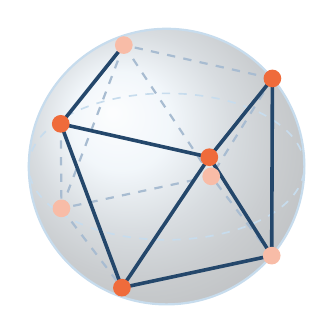
\begin{tikzpicture}
      \shade[ball color=plsky!35, opacity=0.35] (0,0) circle (1.75cm);
      \draw[plrule, line width=0.8pt] (0,0) circle (1.75cm);
      \draw[plrule, line width=0.6pt, dashed] (0,0) ellipse (1.75cm and 0.93cm);
      \draw[plblue!45, line width=0.8pt, dashed] (1.344,1.119) -- (-0.543,1.543);
      \draw[plblue!45, line width=0.8pt, dashed] (0.567,-0.124) -- (-1.335,-0.531);
      \draw[plblue!45, line width=0.8pt, dashed] (1.344,1.119) -- (0.567,-0.124);
      \draw[plblue!45, line width=0.8pt, dashed] (-1.335,-0.531) -- (-0.567,-1.538);
      \draw[plblue!45, line width=0.8pt, dashed] (-0.543,1.543) -- (-1.335,-0.531);
      \draw[plblue!45, line width=0.8pt, dashed] (-0.543,1.543) -- (0.567,-0.124);
      \draw[plblue!45, line width=0.8pt, dashed] (-1.344,0.543) -- (-1.335,-0.531);
      \draw[plblue!45, line width=0.8pt, dashed] (1.335,-1.131) -- (0.567,-0.124);
      \draw[plnavy, line width=1.3pt, line join=round] (1.344,1.119) -- (1.335,-1.131);
      \draw[plnavy, line width=1.3pt, line join=round] (-0.543,1.543) -- (-1.344,0.543);
      \draw[plnavy, line width=1.3pt, line join=round] (-1.344,0.543) -- (0.543,0.119);
      \draw[plnavy, line width=1.3pt, line join=round] (-0.567,-1.538) -- (1.335,-1.131);
      \draw[plnavy, line width=1.3pt, line join=round] (-1.344,0.543) -- (-0.567,-1.538);
      \draw[plnavy, line width=1.3pt, line join=round] (0.543,0.119) -- (1.344,1.119);
      \draw[plnavy, line width=1.3pt, line join=round] (0.543,0.119) -- (1.335,-1.131);
      \draw[plnavy, line width=1.3pt, line join=round] (0.543,0.119) -- (-0.567,-1.538);
      \fill[plorange!45] (0.567,-0.124) circle (3.2pt);
      \fill[plorange!45] (-1.335,-0.531) circle (3.2pt);
      \fill[plorange!45] (-0.543,1.543) circle (3.2pt);
      \fill[plorange!45] (1.335,-1.131) circle (3.2pt);
      \fill[plorange] (1.344,1.119) circle (3.2pt);
      \fill[plorange] (-0.567,-1.538) circle (3.2pt);
      \fill[plorange] (-1.344,0.543) circle (3.2pt);
      \fill[plorange] (0.543,0.119) circle (3.2pt);
    \end{tikzpicture}

      \vspace{6pt}
      {\plmeta\color{plmuted}The square antiprism, $N = 8$\par}
    \end{column}

  \end{columns}
  \vfill
\end{frame}

\end{document}
